\documentclass{article}
\usepackage[T1]{fontenc}
\usepackage[utf8]{inputenc}
\usepackage{hyperref}
\usepackage{graphicx}
\usepackage{caption}
\usepackage{subcaption}
\usepackage{array}
\usepackage{geometry}

\usepackage{biblatex}
\addbibresource{references.bib}

\title{Assignment \#1 report}

\author{\textbf{Student:} Isac Pasianotto}
\date{2024-05}

\setcounter{section}{-1} % Start chapter numbering from 0
\renewcommand{\thesection}{\arabic{section}} % Adjust section numbering in the table of contents

\begin{document}
    \maketitle
    %\tableofcontents

    \section{Requirements}\label{sec:requirements}

    The aim this assignment is to (try to) reproduce the experiment reported in \textit{"Figure 1."}
    of the paper \cite{Rumelhart1986LearningRB}.

    That consist in implementing a small neural network to solve the following classification task:
    given a 6-bit long binary number as input, determine if this is palindromic number or not.

    \section{Network definition}\label{sec:network-definition}

    The network described in the paper was composed by a neuron in the input layer for each digit of
    the number (i.e. six neurons in total), two neurons in the unique hidden layer and just one neuron
    in the output layer.

    \noindent The authors provided also a figure (reported in ~\ref{fig:1.A}) of the network, which we can
    redraw with a more conventional representation as ~\ref{fig:1.B}.


    \begin{figure}
        \centering
        \begin{subfigure}[b]{0.45\textwidth}
            \centering
            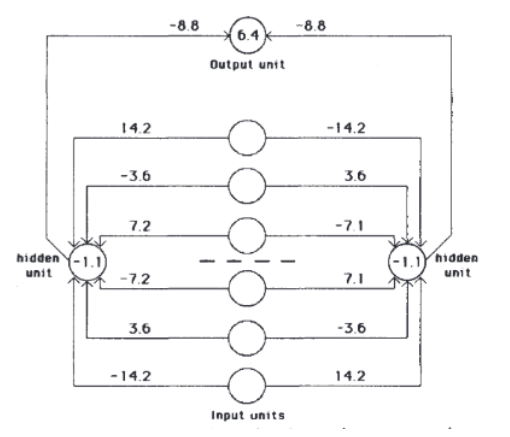
\includegraphics[width=\textwidth]{images/img-01}
            \caption{Network representation presented in the paper.}
            \label{fig:1.A}
        \end{subfigure}
        \begin{subfigure}[b]{0.45\textwidth}
            \centering
            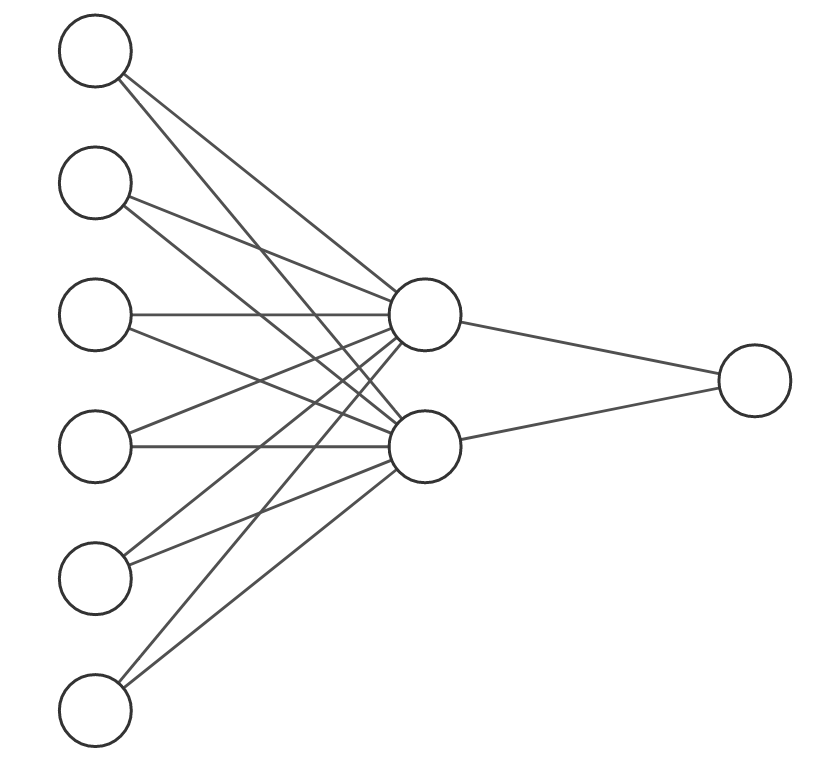
\includegraphics[width=\textwidth]{images/img-00}
            \caption{Network representation with a more conventional layout.}
            \label{fig:1.B}
        \end{subfigure}
        \caption{Network used in the experiment: 6 input neurons, 2 hidden neurons and 1 output neuron.}
        \label{fig:1}
    \end{figure}


    Moreover, the authors provided the following additional information about the network:

    \begin{itemize}
        \itemsep0em % Reduce space between items
        \item The initial weights of the network were randomly chosen from a uniform distribution in the range $[-0.3,\ 0.3]$.
        \item They use the whole dataset (64 combinations of 6-bit binary numbers) to train the network.
        \item The used loss function was $E = \frac{1}{2}\sum_{c}\sum_{j}{\left(y_{i,c} - d_{i,c}\right)^2}$.
        \item The learning rate was set to $\eta = 0.1$ and the number of epochs the train lasted was 1,425.
    \end{itemize}

    What is missing in the paper is:

    \begin{itemize}
        \itemsep0em % Reduce space between items
        \item The activation function used in the hidden and output layers.
            I assumed that the authors used the sigmoid function,since it was the only one mentioned in the paper.
        \item The initializations of the bias terms.
            I assumed that they were initialized with zero.
    \end{itemize}

    \section{Results}\label{sec:results}

    Performing the experiment, trying to still as close as possible to the original formulation didn't lead
    to a very promising result, as shown in the figure ~\ref{fig:2}.

    \noindent I blame the unbalanced dataset for the unsatisfactory results, since the number of palindromic numbers is much smaller
    of the non-palindromic ones.
    In fact even if the accuracy seems to be good, this is due to the fact that the network
    ended up into being a dummy classifier, always predicting the most frequent class.

    \noindent Considering a balanced dataset (repeating the palindromic numbers more than once to match the number of non-palindromic numbers)
    lead to a much better result, as shown in the figure ~\ref{fig:3}.

    Since we were encouraged to try different variations of the experiment, I tried to train the network in several ways, which can be summarized in the table ~\ref{tab:1}.

    \begin{table}
        \footnotesize
        \centering
        \begin{tabular}{ p{2.6cm} p{1.5cm} p{1.5cm} p{1.5cm} p{1.5cm} p{1.5cm} p{1.5cm} p{1.5cm} }
            \hline
            \textbf{description} & \textbf{balanced dataset} & \textbf{learning rate} & \textbf{hidden neurons} & \textbf{loss Function} & \textbf{activation Function} & \textbf{optimizer} & \textbf{figure}\\
            \hline
            Original experiment & no & 0.1 & 2 & $E$ & sigmoid & GD & ~\ref{fig:2}\\
            Balanced dataset & yes & 0.1 & 2 & $E$ & sigmoid & GD & ~\ref{fig:3}\\
            double learning rate & no & 0.2 & 2 & $E$ & sigmoid & GD & ~\ref{fig:4}\\
            halved learning rate & no & 0.05 & 2 & $E$ & sigmoid & GD & ~\ref{fig:5}\\
            4 hidden neurons & no & 0.1 & 4 & $E$ & sigmoid & GD & ~\ref{fig:6}\\
            softmargin loss & no & 0.1 & 2 & softmargin & sigmoid & GD & ~\ref{fig:7}\\
            ReLU activation & no & 0.01 & 2 & $E$ & ReLU & GD & ~\ref{fig:8}\\
            Adam optimizer & no & 0.01 & 2 & $E$ & sigmoid & Adam & ~\ref{fig:9}\\
            \hline
        \end{tabular}
        \caption{Summary of the experiments.}
        \label{tab:1}
    \end{table}

    \newpage
    \section{Variations on the original experiment}\label{sec:variations}

    \begin{figure}
        \centering
        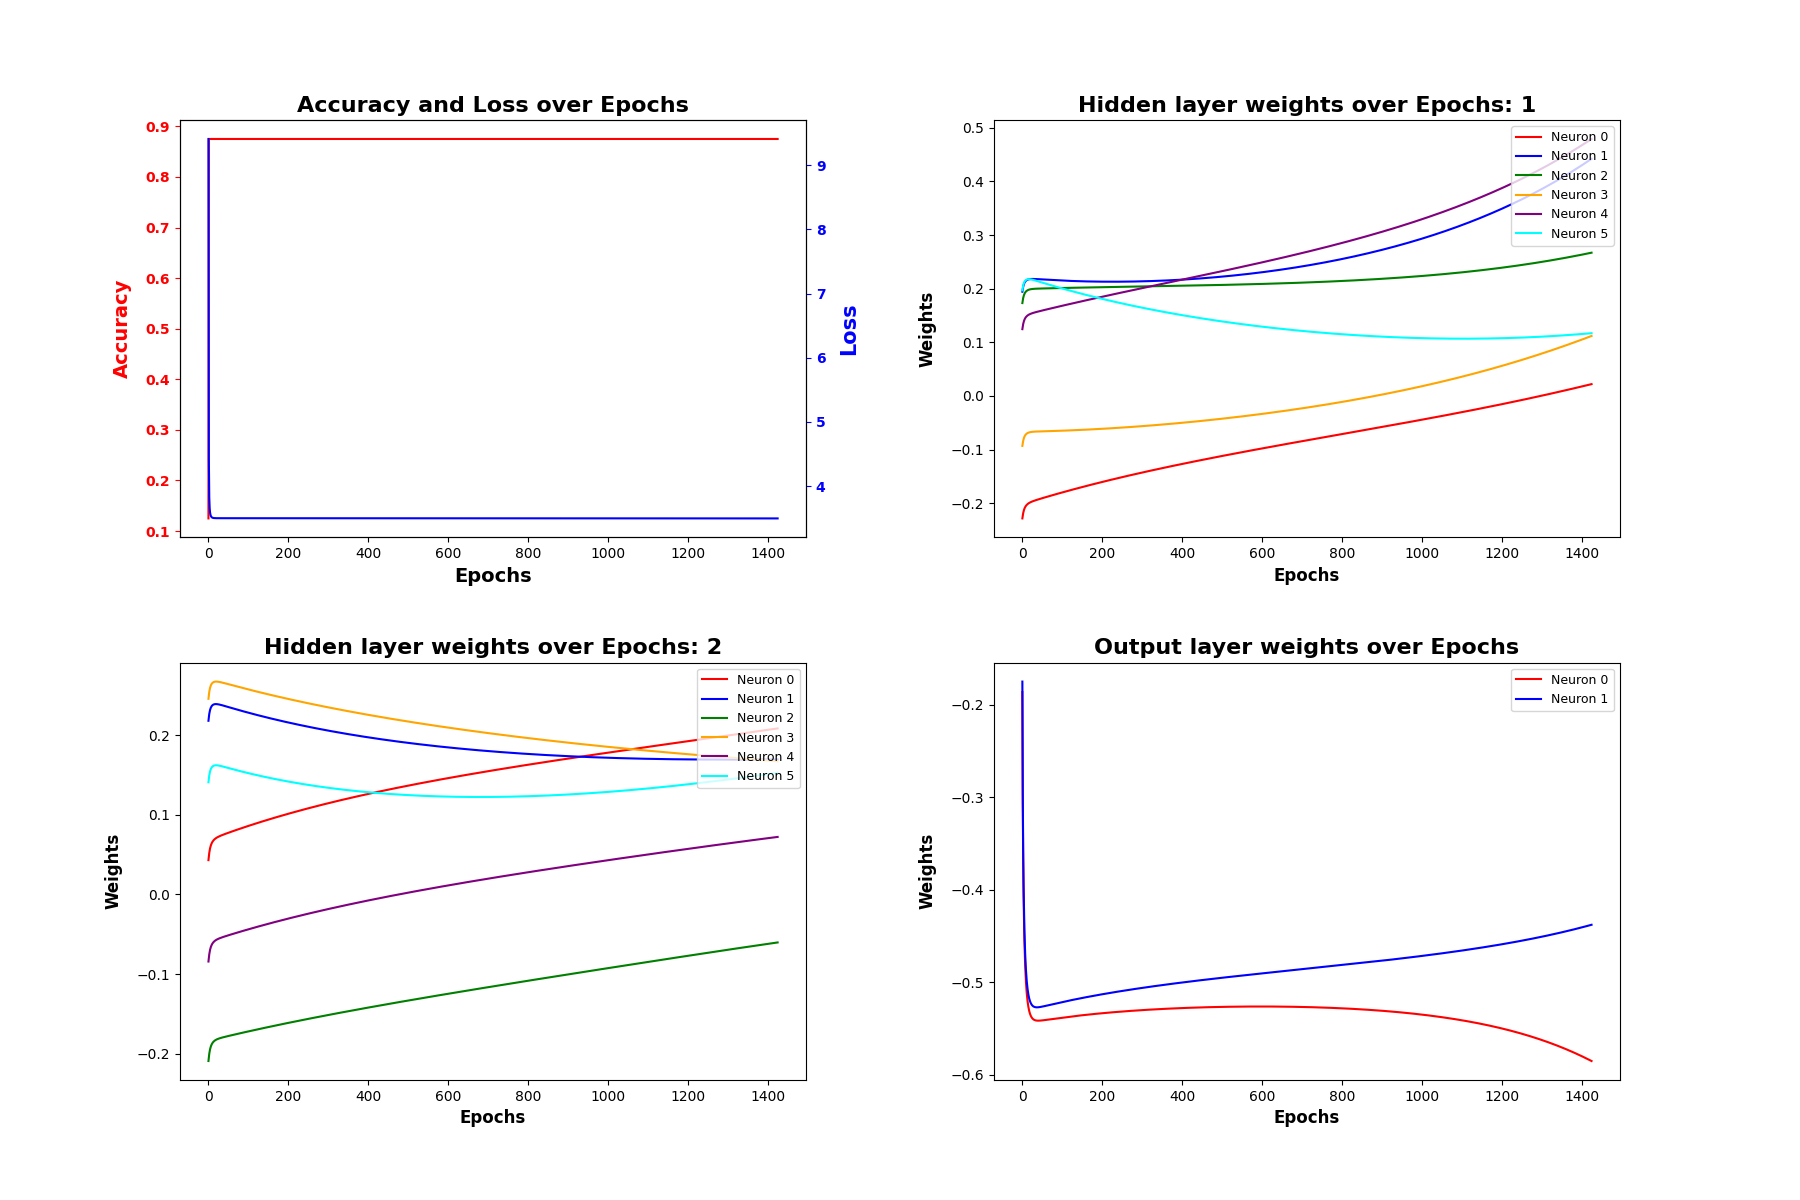
\includegraphics[width=0.8\textwidth]{images/plt-00}
        \caption{Original experiment results.}
        \label{fig:2}
    \end{figure}

    \begin{figure}
        \centering
        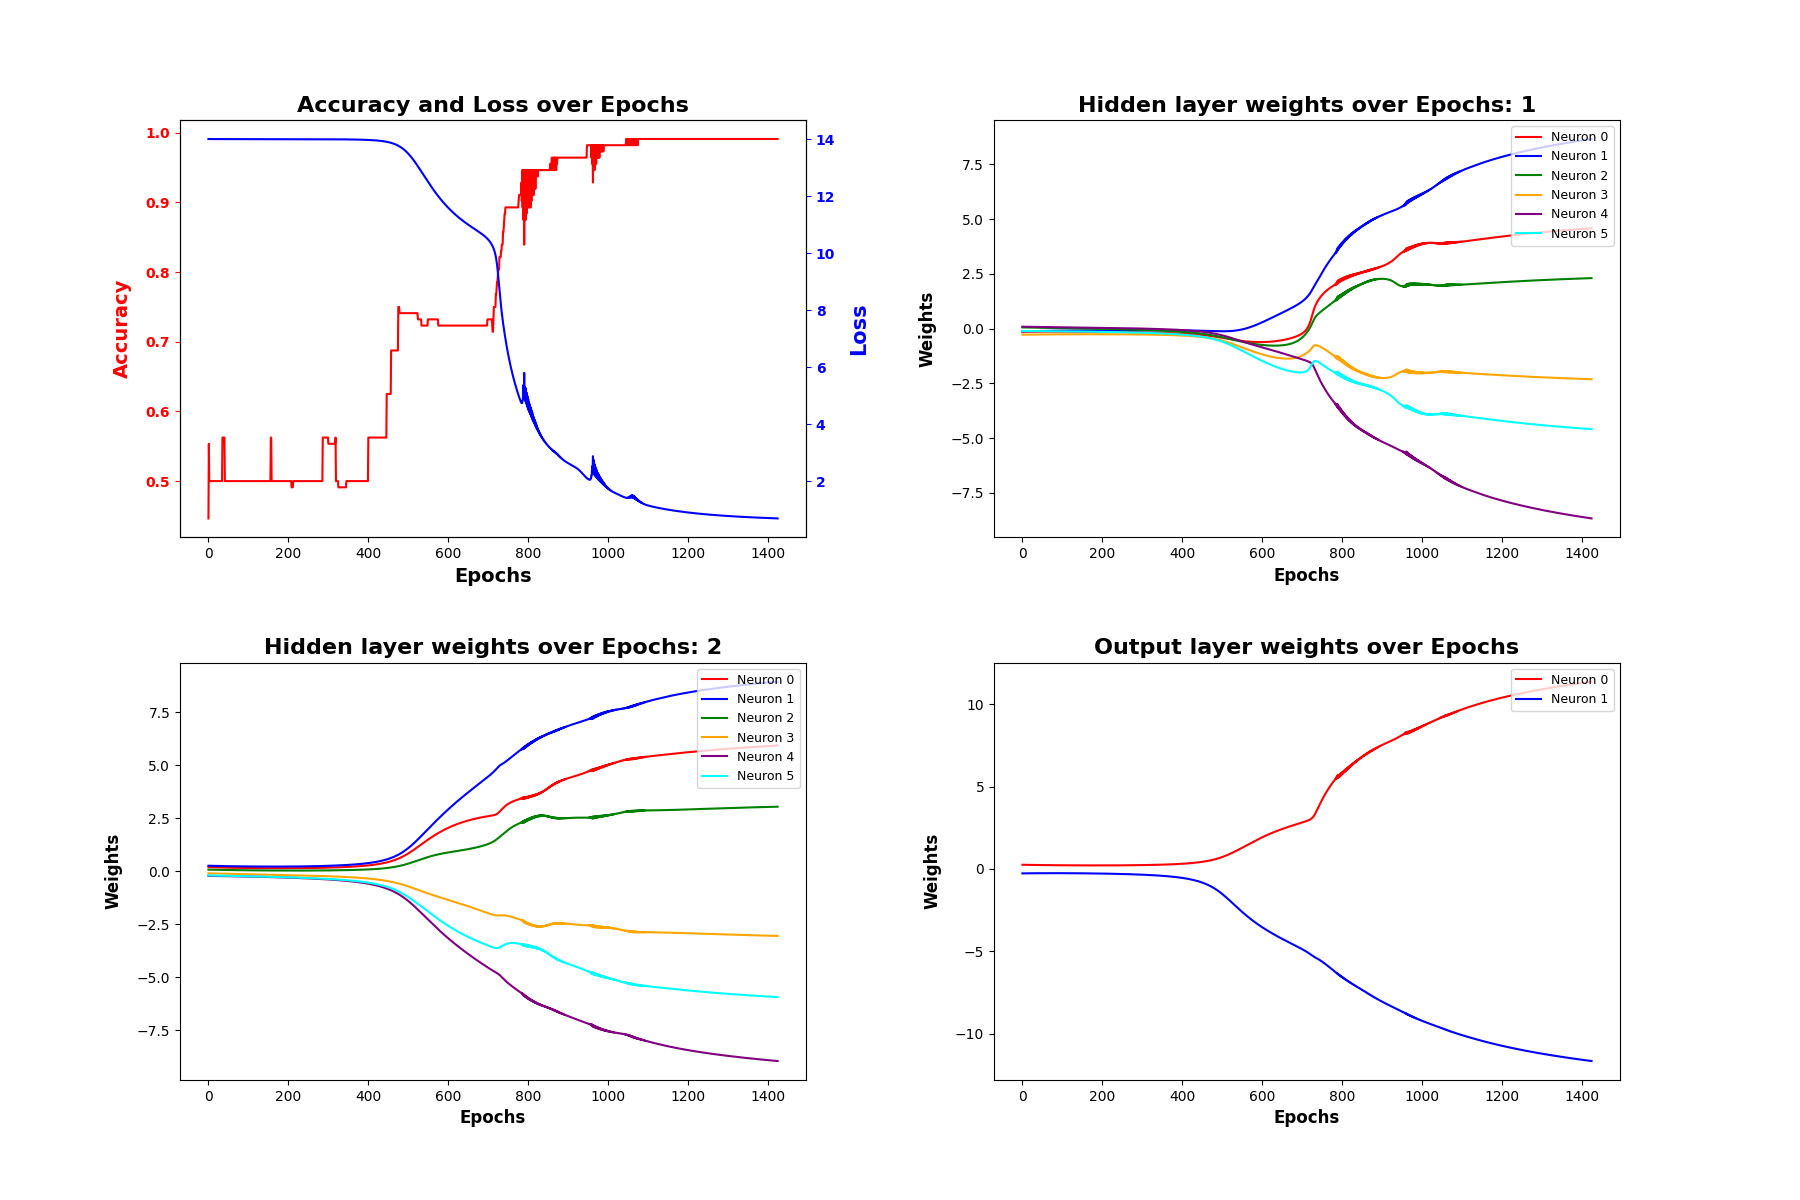
\includegraphics[width=0.8\textwidth]{images/plt-01}
        \caption{Original network, but with a balanced dataset.}
        \label{fig:3}
    \end{figure}

    \begin{figure}
        \centering
        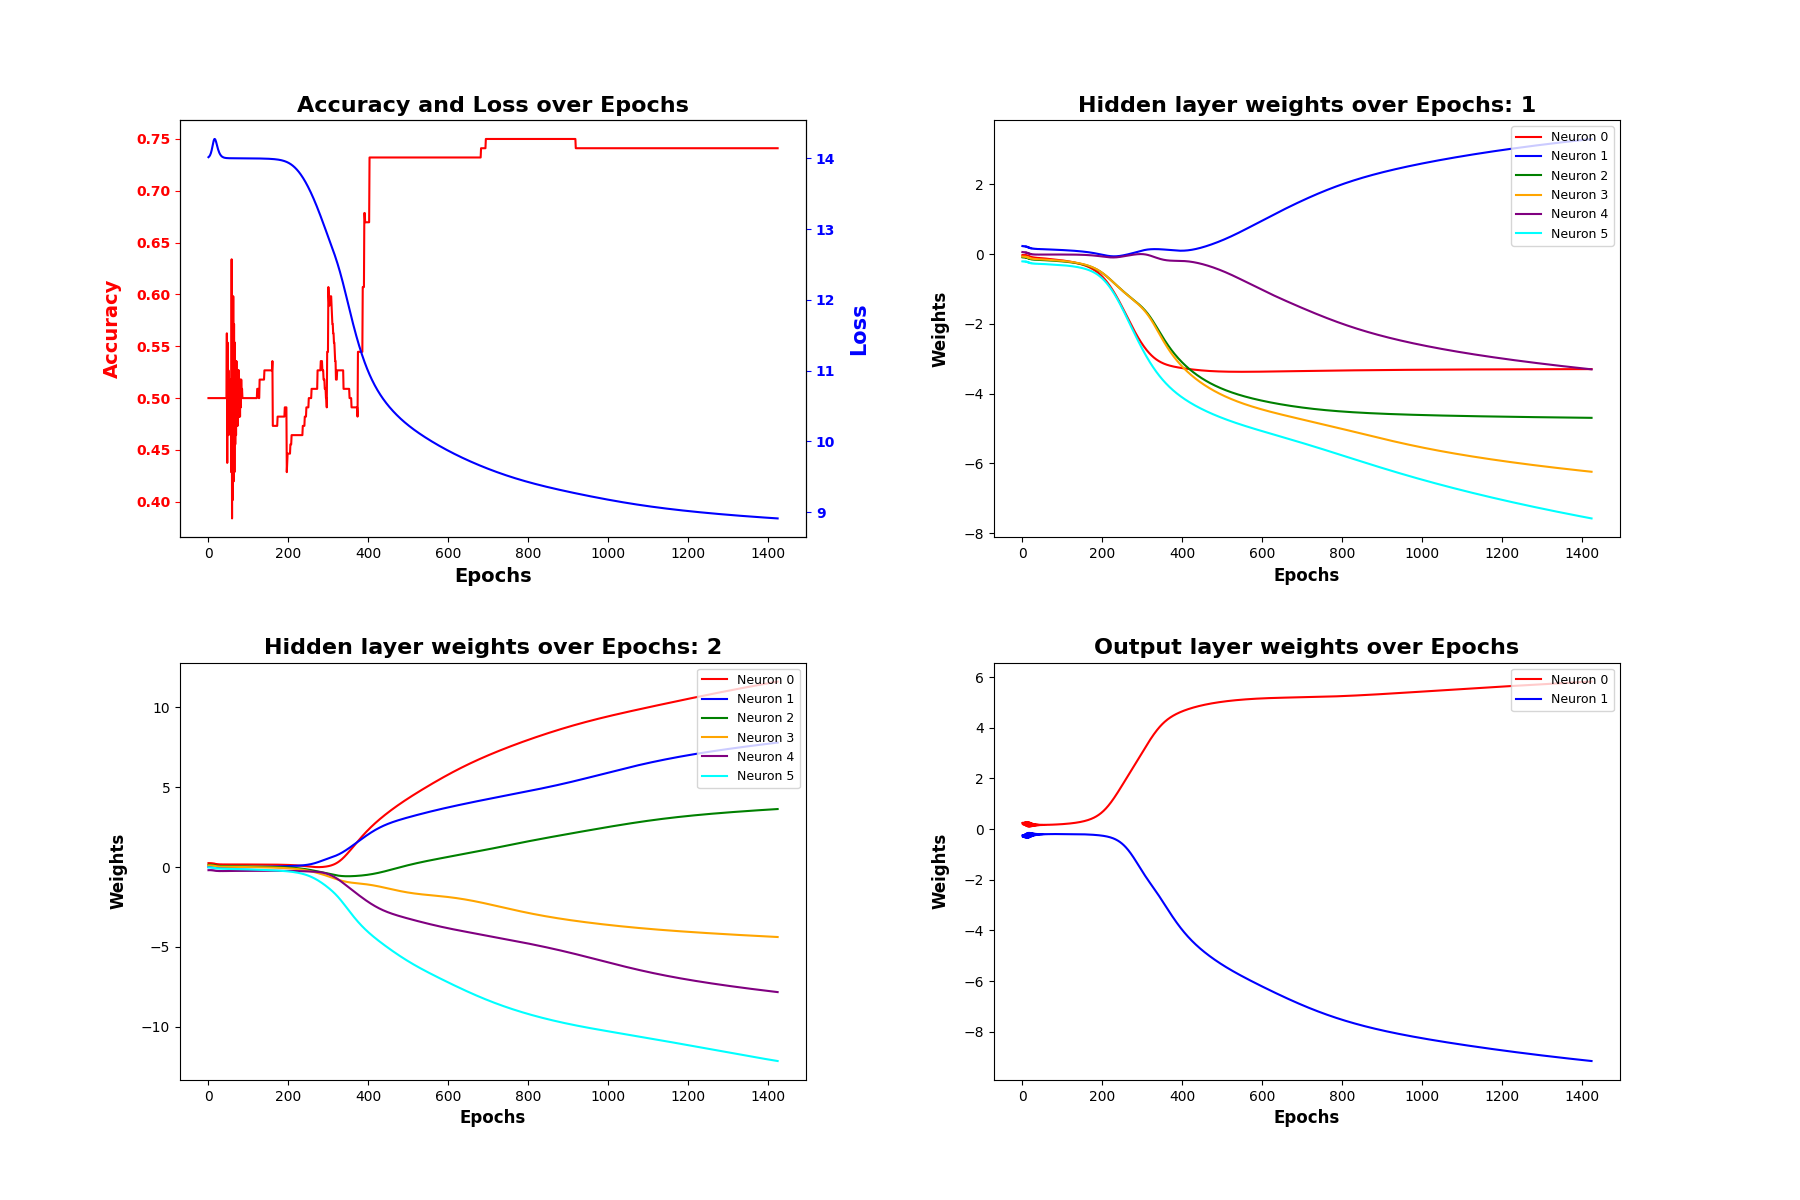
\includegraphics[width=0.8\textwidth]{images/plt-02}
        \caption{Original network, but with doubled learning rate.}
        \label{fig:4}
    \end{figure}

    \begin{figure}
        \centering
        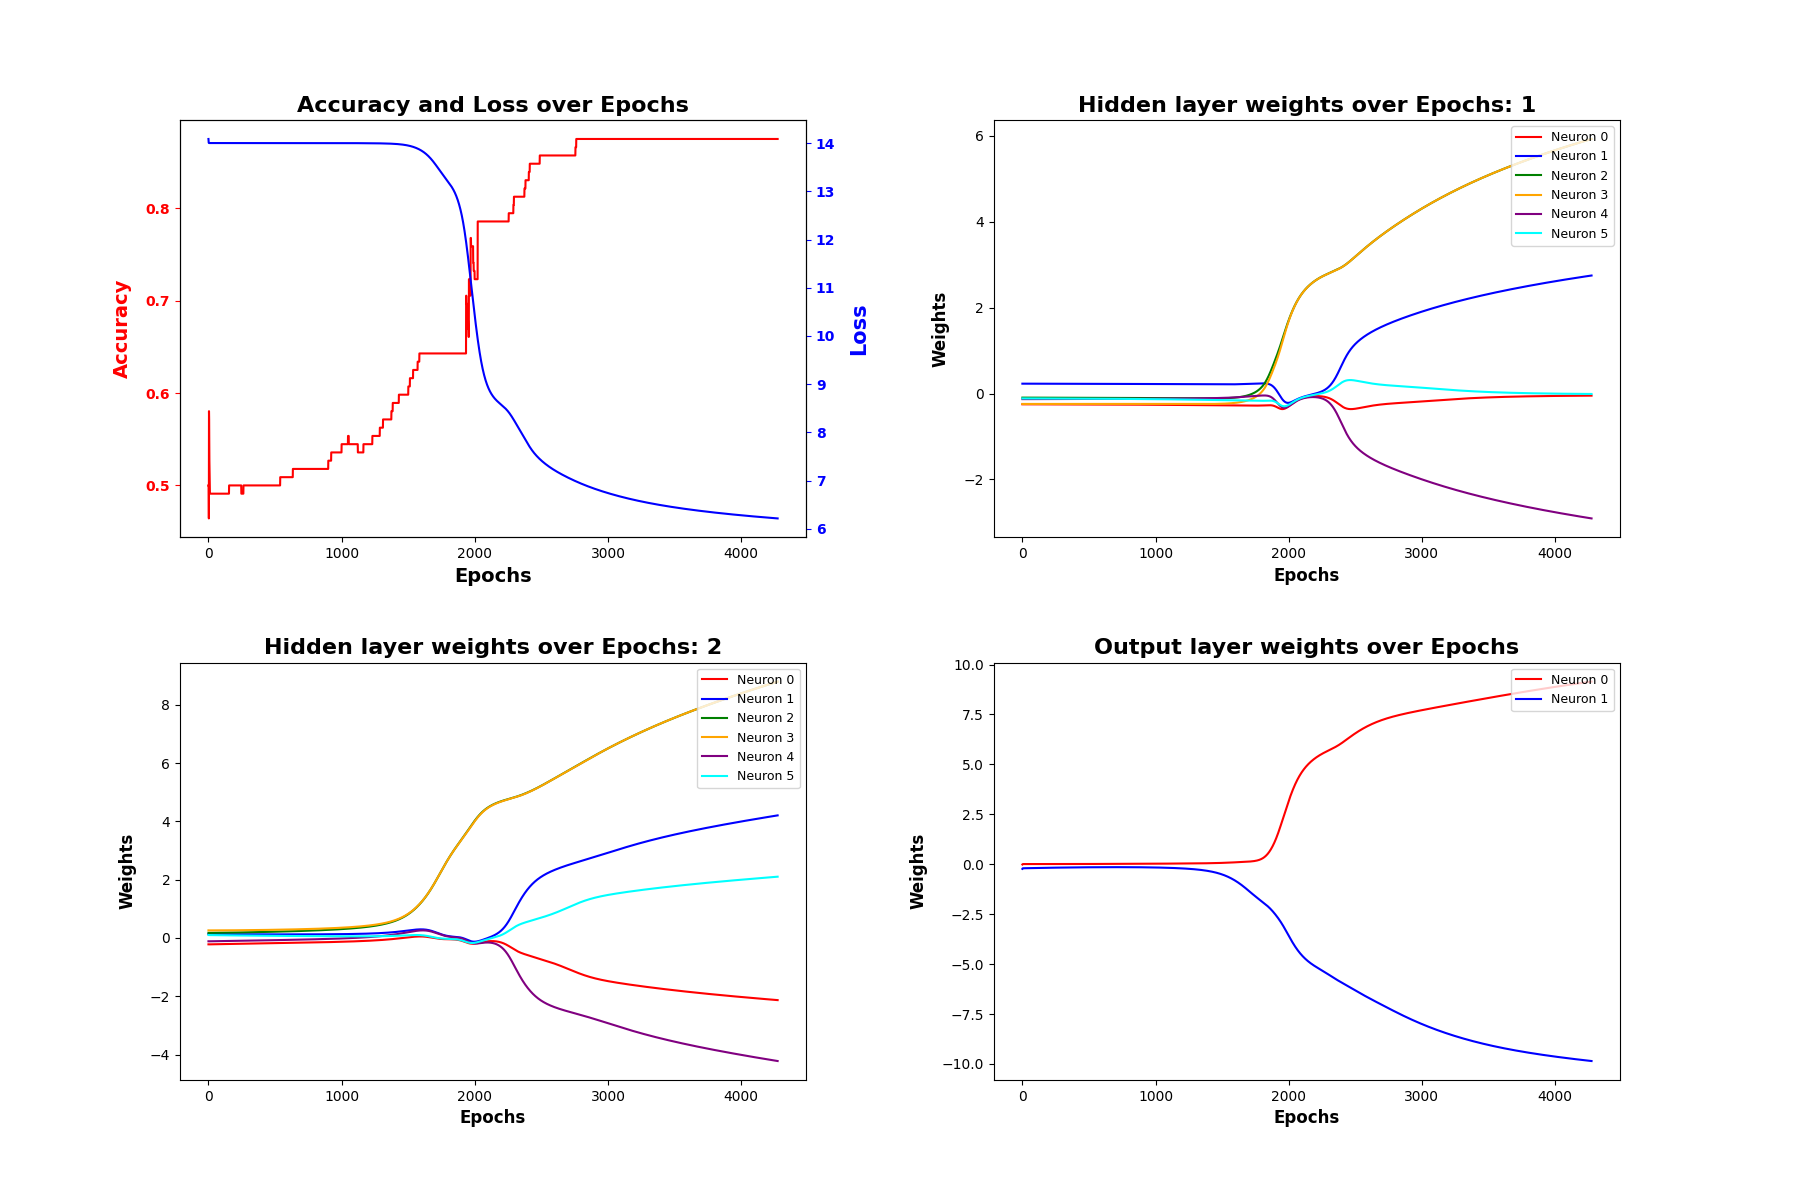
\includegraphics[width=0.8\textwidth]{images/plt-02-bis}
        \caption{Original network, but with halved learning rate.}
        \label{fig:5}
    \end{figure}

    \begin{figure}
        \centering
        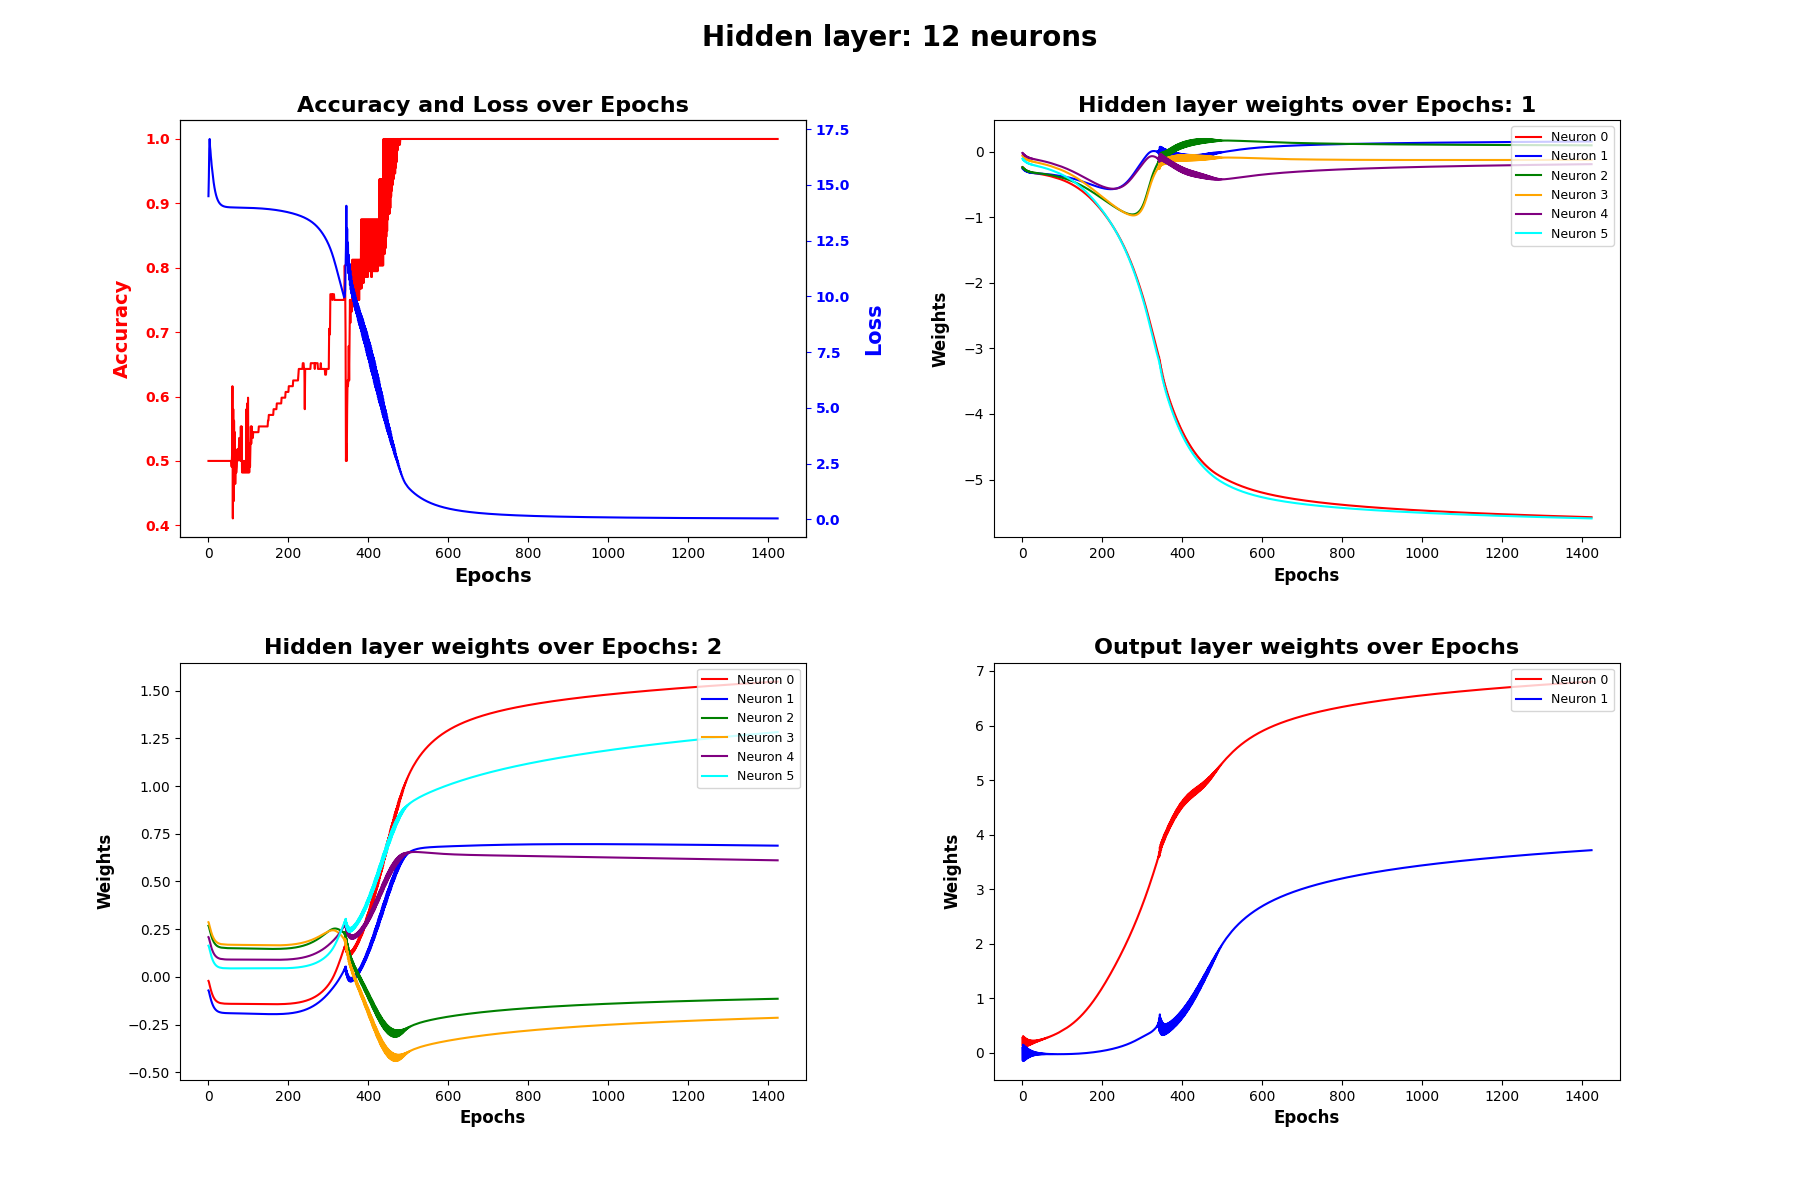
\includegraphics[width=0.8\textwidth]{images/plt-03}
        \caption{Network with 4 hidden neurons. In the plot are reported only the hidden layer weights of the first 2 neurons.}
        \label{fig:6}
    \end{figure}

    \begin{figure}
        \centering
        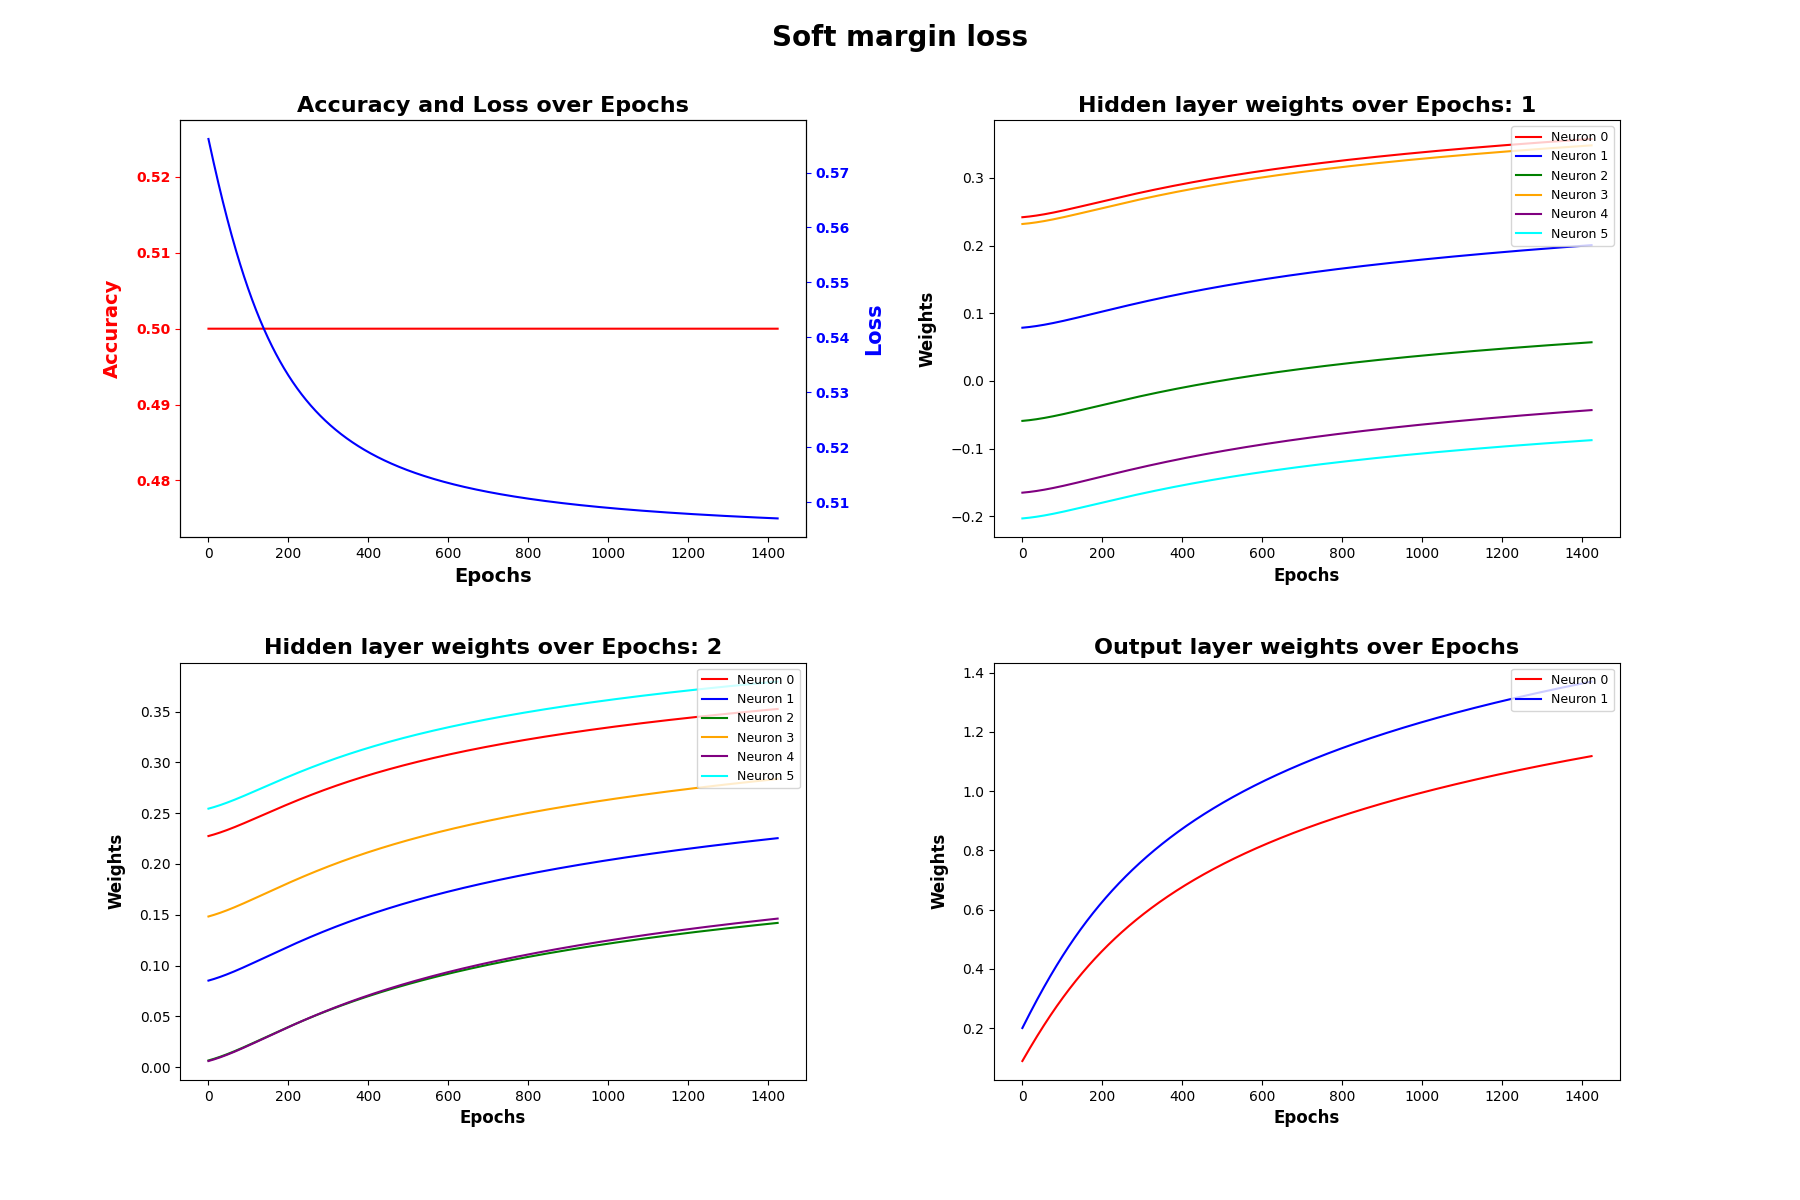
\includegraphics[width=0.8\textwidth]{images/plt-04}
        \caption{Original network, but using the softmargin loss function.}
        \label{fig:7}
    \end{figure}

    \begin{figure}
        \centering
        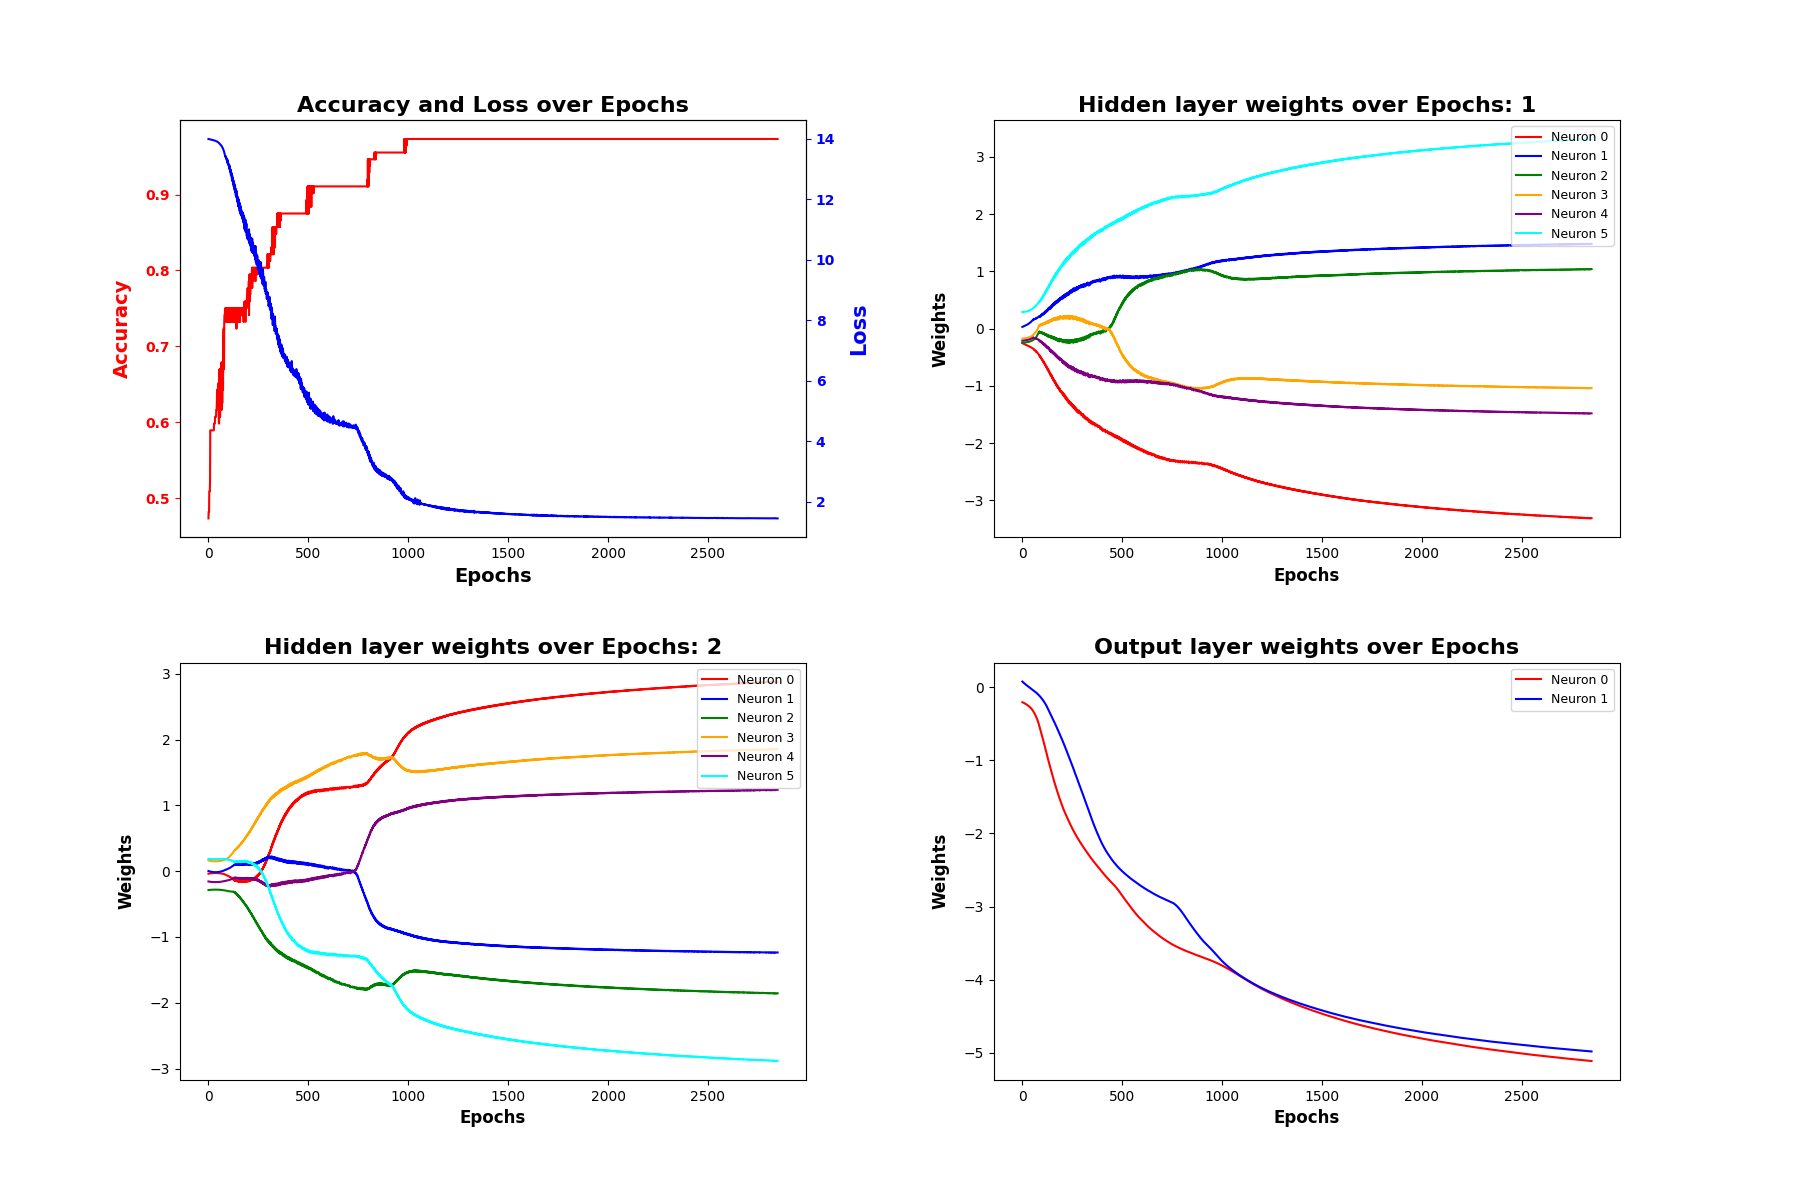
\includegraphics[width=0.8\textwidth]{images/plt-05}
        \caption{Network in which the hidden layer has the ReLU activation function.}
        \label{fig:8}
    \end{figure}

    \begin{figure}
        \centering
        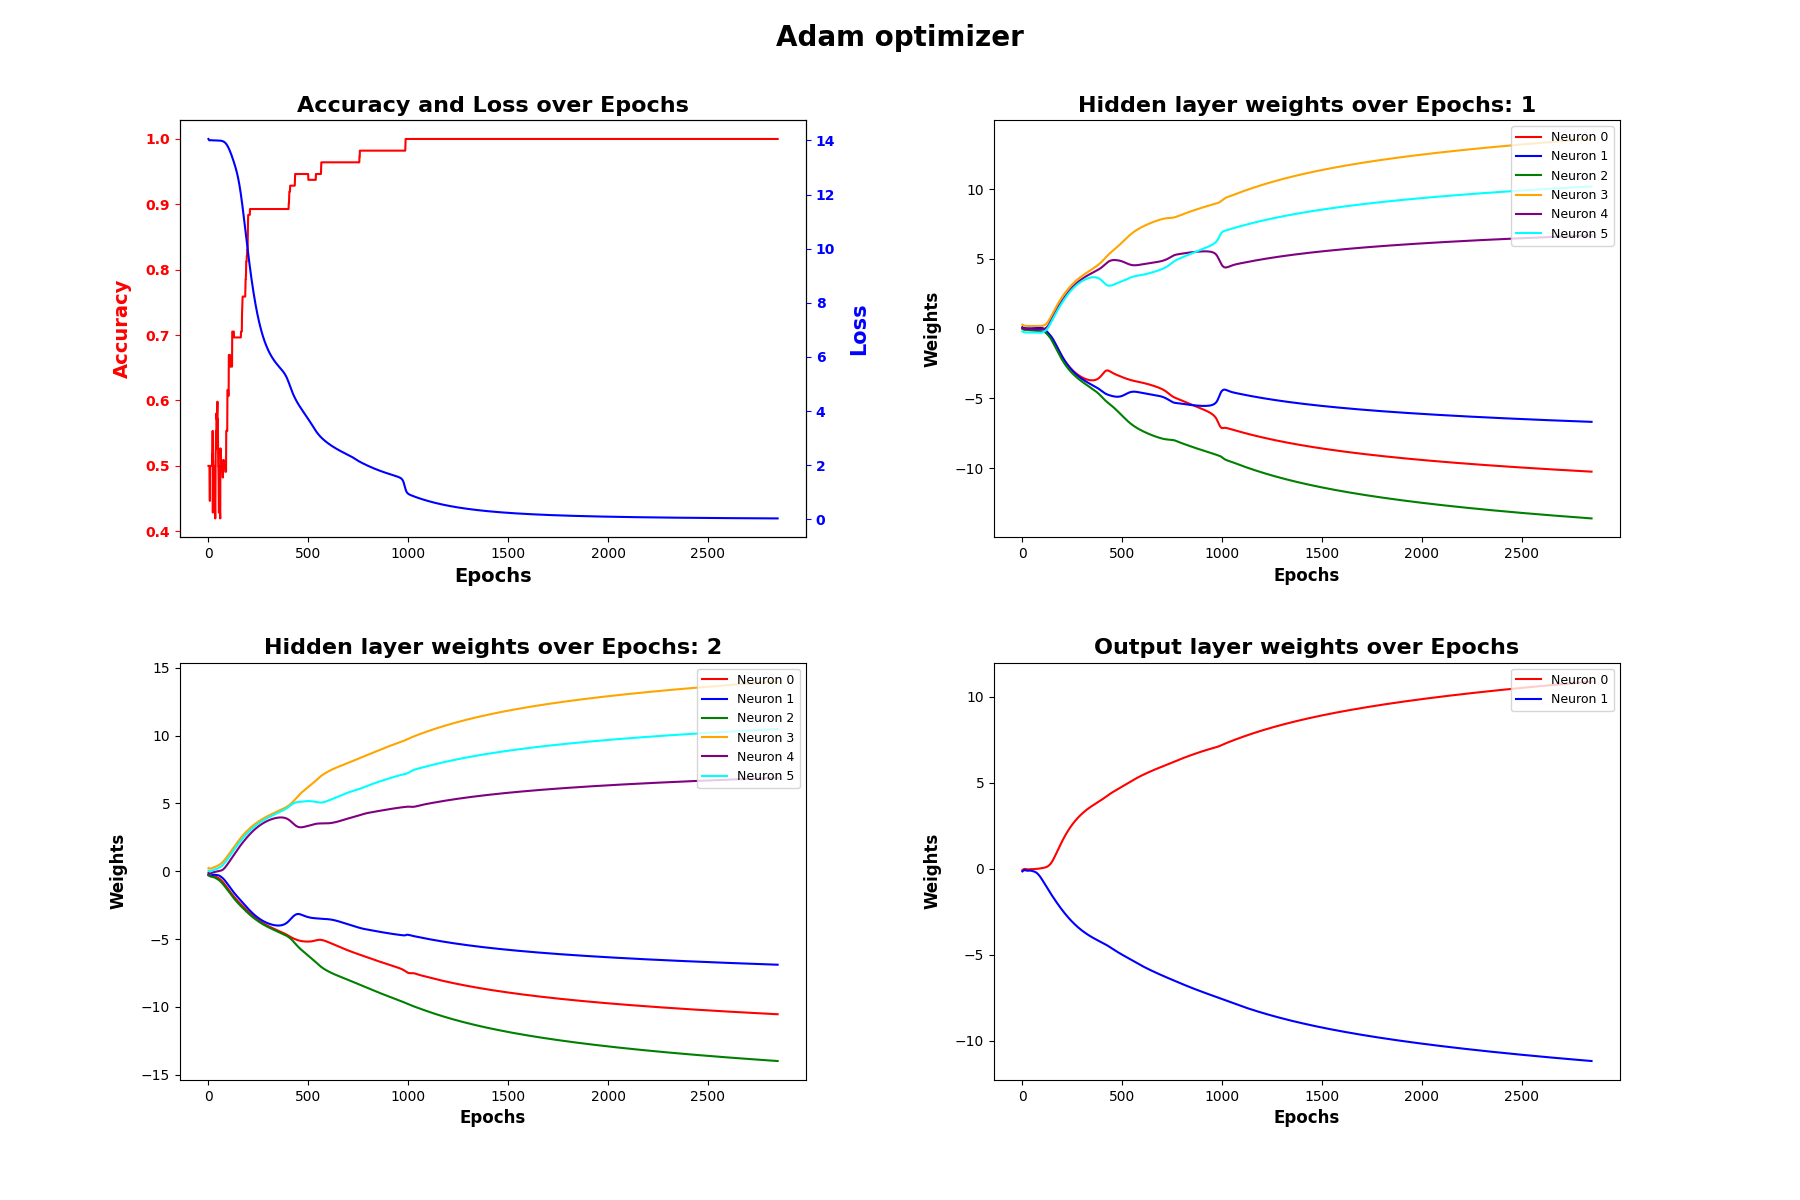
\includegraphics[width=0.8\textwidth]{images/plt-06}
        \caption{Original network architecture, but using the Adam optimizer.}
        \label{fig:9}
    \end{figure}

    \newpage
    \medskip
    \printbibliography

\end{document}